\section{Schedule Memoization}  \label{sec:tern-batch}

This section presents the idea of schedule memoization in the context of
batch programs.  We describe how \tern memoizes schedules
(\S\ref{sec:tern-derive-schedule}), tracks input constraints
(\S\ref{sec:tern-track-constraints}), merges a schedule into the schedule cache
(\S\ref{sec:tern-schedule-cache}), and reuses schedules
(\S\ref{sec:tern-reuse-schedule}).

\subsection{Memoizing Schedules}  \label{sec:tern-derive-schedule}

To memoize schedules, the memoizer controls and logs synchronization
operations. By default, it uses a simple round-robin (RR) algorithm that
forces each thread to do synchronizations in turn.  One advantage of this
algorithm is that independent sites may memoize the same schedules, making
program behaviors deterministic and stable across sites.

\begin{figure}[t]
\lgrindfile{tern/code/memoize.cpp.lineno}
\caption{\small \emph{The memoizer's round-robin scheduling algorithm.}}
\label{fig:tern-memoizer}
\end{figure}

The memoizer implements this algorithm by implementing the wrapper
functions in Table~\ref{tab:tern-interface}.  Figure~\ref{fig:tern-memoizer} shows
the wrappers to \vv{pthread\_mutex\_lock()} and
\vv{pthread\_mutex\_unlock()}.  The memoizer maintains a queue of active
threads.  Only the thread at the head of the queue ``has the turn'' (line
4 and 14).  Once the thread is done with the operation, it gives up the
turn by moving itself to the tail of the queue (line 7 and 18).

We explain three subtleties of the code.  First, to avoid the deadlock
scenario when the head of the queue attempts to grab an unavailable mutex,
we call the non-blocking lock operation instead of the blocking one (line
5).  If the mutex is not available, the thread gives up its turn and waits
on a \tern-maintained wait queue (line 10).  \tern uses its own wait queues
to avoid nondeterministic wakeup orders in pthread library.  Second, we
log synchronizations (line 6 and line 17) only when the thread has the turn, so
that the log faithfully reflects the actual order of synchronizations.
Lastly, we maintain our internal thread IDs to avoid nondeterminism in the
OS thread IDs across runs.  Function \vv{self()} returns this internal ID
for the current thread (line 6 and line 17).

The memoizer allows a thread to break out of the round-robin when the
thread has waited for its turn for over a second.  The rationale is that
if a thread has waited too long, the current schedule will likely
perform poorly in reuse runs.  However, such timeouts do not affect
nondeterminism, because the memoizer still logs the order of the occurred
operations and the replayer simply enforces the same order.  In our
experiments, we never observed such timeouts because most threads
synchronize or call blocking system calls frequently.

Unlike previous \dmt systems, \tern has the flexibility to select
scheduling algorithms.  In addition to the RR algorithm, it implements a
first-come first-served (FCFS) algorithm that lets threads run as is.  If
the memoizer detects a race using RR, it can restart the run and 
switch to FCFS.  Implementing
FCFS requires only minor modifications to the algorithm presented in
Figure~\ref{fig:tern-memoizer}. Specifically, we replace line 4 and line 14
with a lock operation; line 7, line 10, and line 18 with an unlock
operation; and line 16 a NOP.

%% The memoizer handles other synchronization operations similar to lock and
%% unlock with the most involved one being \vv{pthread\_cond\_wait()}.
%% %  and \vv{pthread\_create()}.  
%% For brevity, we omit the details and only note that we replace the mutex
%% used in a \vv{pthread\_cond\_wait()} call with our own mutex to avoid
%% potential deadlocks and maintain an internal queue to ensure that threads
%% waiting on the condition variable are woken up in a deterministic order.
%% signal becomes broadcast

%and refer interested readers to our identically titled technical report.

In addition to synchronizations, the memoizer includes the hooks around
blocking system calls (\S\ref{sec:tern-annotations})
in the schedule it memoizes because blocking system calls are natural
scheduling points.  However, the replayer will only opportunistically
replay these hooks when reusing a schedule because the returns from
blocking system calls are driven by the program's environment.


%     why simpler than kendo?

%         our wait for turn is just RR, not based on logical clock

%    log contains only successful operations, because don't want to replay
%    failed operations.

%    how to implement try lock?
%       treat as lock
%       if always fail, may be a problem.

%%   cond wait:

%%    acquire and release.  must give up turn before wait.  
%%    difficult.  can have nondeterminism  such as

%%    wait for turn
%%                              wait for turn
%%    try lock
%%                              give up turn
%%                              cond wait


%%    fix:

%%    wait for turn

%%    wake up waiting on signal
   
   
   
   
%%                              wait for turn
%%                              // mark lock available
%%                              // mark wait on signal and mutex

%%                              give up turn and wait on signal

%%                              cond wait (cv, fake m);

%%                              wrap lock();

%%                              wait for turn

%%                              try lock
%%                                log
%%                                give up turn
%%                              els
%%                                wait on lock;


%%   pthread create: 

%%     maintain own thread IDs to avoid nondeter

%%     deterministic child id

%%     create thread suspended

%%     after getting real id of child
    
%%     wake up child



\subsection{Tracking Input Constraints} \label{sec:tern-track-constraints}

Given the symbolic data marked by developers, the memoizer tracks the
constraints on this data by tracking (1) what data is derived from the
symbolic data and (2) the outcomes of the branch statements that observe this
symbolic and derived data.  At the end of this memoization run, the set of
branch outcomes together describe the constraints to place on the symbolic
data required to reuse the memoized schedule.  That is, if an input
satisfies these constraints, we can re-run the program in the same way as
the memoization run.  The constraints collected this way may be
over-constraining if developers annotate too much data as symbolic.  We
describe a technique to address this problem in \S\ref{sec:tern-slicing}.

\tern leverages \klee~\cite{klee:osdi08}, an open-source symbolic execution
engine to track input constraints.  To adapt \klee to \tern, we made two key
modifications.  First, \klee works only with sequential programs, thus we
extended it to support threads.  Specifically, we modified \klee to spawn a
new \klee instance for each new thread.  At the end of the run, we unify
the constraints collected from each thread as the input constraints of the
schedule.  Second, we simplified \klee to only collect constraints without
solving them, because unlike \klee, \tern need not explore different
execution paths.

% \klee is designed to
% generate many different testcases to test many paths.  The original \klee
% solves constraints to explore different execution paths of a program, and
% constraint solving can be expensive and unnecessary for the memoizer.
% It does so by
% systematically exploring both branches of a symbolic conditional, which
% involves much (slow) constraint solving.  
%% Third, due to a limitation of the constraint solver \klee uses, it
%% concretizes symbolic divisions (either the divisor or the dividend is
%% symbolic) when divisor is not a power of two.  We modified \klee to simply
%% ignore symbolic divisions.  
%% Lastly, we extended \klee to track both symbolic and concrete values for
%% symbolic inputs so that we can concretize the symbolic inputs with
%% meaningful values (cf \S\ref{sec:window}).

% it will bring us down the same code path in each thread.


%% For instance, they may mark all
%% command line arguments as symbolic when in fact most arguments do not
%% affect schedules.  

\subsection{Merging Schedules into the Schedule Cache} \label{sec:tern-schedule-cache}

\begin{figure}[t]
\begin{center}
\includegraphics[width=0.4\textwidth]{tern/figures/cache.eps}
\end{center}
\caption{\emph{Decision tree of \tern's schedule cache.}}
\label{fig:tern-schedule-tree}
\end{figure}

Once \tern memoized a schedule $S$ and its constraints $C$, \tern stores the
tuple into the schedule cache.  Although the schedule cache is
conceptually a set of $\langle C, S \rangle$ tuples, its actual structure
is a decision tree because a program may incrementally read inputs from
its environment, calling \vv{symbolic()} multiple times.  For example, the
code in Figure~\ref{fig:tern-pbzip2} calls \vv{symbolic()} twice.

Figure~\ref{fig:tern-schedule-tree} illustrates how \tern constructs the
decision tree of the schedule cache.  Given a $\langle C, S \rangle$
tuple, \tern breaks it down to sub-tuples $\langle C_i, S_i \rangle$
separated by \vv{symbolic()} calls, where $S_i$ contains the
synchronization operations logged and $C_i$ contains the constraints
collected between the $i^{th}$ and $(i+1)^{th}$ \vv{symbolic()} calls.  It
then merges the sub-tuples into the $i^{th}$ level of the decision tree.

\tern avoids merging redundant tuples into the cache.  That is, if the
cache contains a tuple with less restrictive constraints that the tuple
being merged, \tern simply discards the new tuple.  Note that the tuples
may overlap (\ie, one input satisfies more than one set of constraints),
and \tern simply returns the first match if there are multiple matches.

To speed up cache lookup, \tern sorts all $\langle C_i, S_i \rangle$ tuples
within the same decision node based on their \emph{reuse rates}, defined
as the number of successful reuses of $S_i$ over the number of inputs that
have satisfied $C_i$.  Reusing a schedule may fail even if the input
satisfies the schedule's input constraints (cf next subsection).  However,
by sorting the tuples based on reuse rates, we automatically prefer good
schedules over bad ones that have many failed reuse attempts.  To bound
the size of the schedule cache, \tern can throw away bad schedules based on
reuse rates.  However, we have not found the need to do so because
the schedule cache is often small.


%% input timing nondeterminism
%%   - blocking system call returns
%%   - asynchronous i/o completion
%%   - signal handlers
%%   simply record.  
%% system may wake up wrong thread
%%   - replay to the right thread
%% blocking wait instead of busy wait.  thread-private semaphore.
%% try lock to check if lock is available.

\subsection{Reusing Schedules} \label{sec:tern-reuse-schedule}

To reuse a schedule, \tern must check that the input satisfies the input
constraints of the schedule.  To do so, it maintains an iterator to the
decision tree of the schedule cache.  The iterator starts from the root.
As the program runs and calls \vv{symbolic()}, \tern moves the iterator down
the tree.  It checks if the data passed into a \vv{symbolic()} call
satisfies any set of constraints stored at the corresponding decision tree
node and, if so, enforces the corresponding schedule.
 
The performance of the replayer is crucial because it runs during a
program's normal executions.  To efficiently enforce a synchronization
order, the replayer uses a technique we call \emph{semaphore relay}.
Specifically, the replayer assigns each thread a semaphore.  Before doing
a synchronization operation, a thread has to wait on its semaphore for its
turn.  Once it is done with the operation, it passes the turn to the next
thread in the schedule by signaling the semaphore of the next thread.
Compared to an approach using locks or condition variables, semaphore
relay avoids unnecessary lock contentions.  Figure~\ref{fig:tern-replayer}
illustrates semaphore relay using the replayer's
\vv{pthread\_mutex\_lock()} wrapper.

\begin{figure}[t]
\begin{minipage}[c]{.8\linewidth}
\tiny \lgrindfile{tern/code/replay.cpp.lineno}
\end{minipage}
\caption{\small \emph{Pseudo code of the replayer}.}
\label{fig:tern-replayer}
\vspace{-.2in}
\end{figure}

We note several subtleties of the pseudo code in
Figure~\ref{fig:tern-replayer}.  First, we do not use non-blocking lock
operations (line 3) as in Figure~\ref{fig:tern-memoizer} because the memoizer only logs successful lock
acquisitions.  Second, the replayer maintains internal thread IDs the same
way as the memoizer to avoid mismatches.  Lastly, the \vv{down()} (line 2)
is actually a timed wait (with a default 0.1ms timeout), so that a
thread can break out of a schedule when the dynamic load mismatches the
schedule's assumptions.  Note that these timeouts merely cause delays and
do not affect correctness.  They rarely occurred in our experiments.






